\documentclass[9pt,twocolumn,twoside,lineno]{pnas-new}
% Use the lineno option to display guide line numbers if required.
% Note that the use of elements such as single-column equations
% may affect the guide line number alignment. 

\templatetype{pnasresearcharticle} % Choose template 
% {pnasresearcharticle} = Template for a two-column research article
% {pnasmathematics} = Template for a one-column mathematics article
% {pnasinvited} = Template for a PNAS invited submission

\title{Template for preparing your research report submission to PNAS using Overleaf}

% Use letters for affiliations, numbers to show equal authorship (if applicable) and to indicate the corresponding author
\author[a,c,1]{Author One}
\author[b,1,2]{Author Two} 
\author[a]{Author Three}

\affil[a]{Affiliation One}
\affil[b]{Affiliation Two}
\affil[c]{Affiliation Three}

% Please give the surname of the lead author for the running footer
\leadauthor{Lead author last name} 

% Please add here a significance statement to explain the relevance of your work
\significancestatement{Authors must submit a 120-word maximum statement about the significance of their research paper written at a level understandable to an undergraduate educated scientist outside their field of speciality. The primary goal of the Significance Statement is to explain the relevance of the work in broad context to a broad readership. The Significance Statement appears in the paper itself and is required for all research papers.}

% Please include corresponding author, author contribution and author declaration information
\authorcontributions{Please provide details of author contributions here.}
\authordeclaration{Please declare any conflict of interest here.}
\equalauthors{\textsuperscript{1}A.O.(Author One) and A.T. (Author Two) contributed equally to this work (remove if not applicable).}
\correspondingauthor{\textsuperscript{2}To whom correspondence should be addressed. E-mail: author.two\@email.com}

% Keywords are not mandatory, but authors are strongly encouraged to provide them. If provided, please include two to five keywords, separated by the pipe symbol, e.g:
\keywords{Keyword 1 $|$ Keyword 2 $|$ Keyword 3 $|$ ...} 

\begin{abstract}
Please provide an abstract of no more than 250 words in a single paragraph. Abstracts should explain to the general reader the major contributions of the article. References in the abstract must be cited in full within the abstract itself and cited in the text.
\end{abstract}

\dates{This manuscript was compiled on \today}
\doi{\url{www.pnas.org/cgi/doi/10.1073/pnas.XXXXXXXXXX}}

\begin{document}

% Optional adjustment to line up main text (after abstract) of first page with line numbers, when using both lineno and twocolumn options.
% You should only change this length when you've finalised the article contents.
\verticaladjustment{-2pt}

\maketitle
\thispagestyle{firststyle}
\ifthenelse{\boolean{shortarticle}}{\ifthenelse{\boolean{singlecolumn}}{\abscontentformatted}{\abscontent}}{}

% If your first paragraph (i.e. with the \dropcap) contains a list environment (quote, quotation, theorem, definition, enumerate, itemize...), the line after the list may have some extra indentation. If this is the case, add \parshape=0 to the end of the list environment.
\dropcap{T}his PNAS journal template is provided to help you write your work in the correct journal format.  Instructions for use are provided below.

Note: please start your introduction without including the word ``Introduction'' as a section heading (except for math articles in the Physical Sciences section); this heading is implied in the first paragraphs. 



%%%%%%%%%%%%%%%%%%%%%%%%%%%%%%%%%%%%%%%%%%%%
\section{Mathematical Definition of the Economic Complexity Index}
\label{sec:ECIdefinition}
The calculation of the ECI starts from the matrix of countries (rows) and the products (columns) they export, $\mtx{M}$. Let this matrix have size $C\times P$. This is a matrix that has been discretized so that $M_{c,p}$ is 1 if the product $p$ is exported in country $c$, and 0 otherwise. From this matrix, one creates two stochastic matrices. First, the right-stochastic (i.e., row-stochastic or row-normalized) transition matrix of ``countries to products'', $$\mtx{R}=\diag{1/\vec{d}}\cdot\mtx{M},$$ and second, the left-stochastic (i.e., column-stochastic or column-normalized) transition matrix of ``products to countries'', $$\mtx{L}=\mtx{M}\cdot\diag{1/\vec{u}},$$ where $\vec{d}=\mtx{M}\cdot\vec{1}$ is the vector that contains the number of products a country exports (i.e., its \emph{diversity}) and where $\vec{u}=\mtx{M}^T\cdot\vec{1}$ is the vector that contains the number of countries from which the product is exported (i.e., its \emph{ubiquity}). We use the notation $\diag{\vec{x}}$ to mean the matrix whose diagonal is the vector $\vec{x}$ and the other values are zero, and $\vec{1}$ to denote a vector of 1's.

Four important characteristics of left-stochastic matrices are worth mentioning, as they will be useful below:\footnote{These properties also hold for right-stochastic matrices, by simply swapping the words ``right'' and ``left''.} 
\begin{enumerate}
    \item A stochastic matrix for discrete markov chain can be represented as a network of nodes connected through directed edges. 
    \item Multiplying on the right of the matrix is the way of \emph{propagating probabilities} through the network of connected nodes. 
    \item Multiplying on the left of the matrix is the way of \emph{averaging some node-specific property} conditioned on standing on each of the nodes and only observing the nodes to which probabilities propagate to.
\end{enumerate}


Let us construct the left-stochastic transition probability matrix of ``countries to countries'', $$\mtx{C}=\mtx{L}\cdot\mtx{R}.$$ For mathematical convenience, we will assume that the stochastic matrix $\mtx{C}$ is irreducible and aperiodic. 

Now, let $\vec{l_i}^T$ and $\vec{r_i}$ be the $i$th left-eigenvector and right-eigenvector, respectively, so that the eigenvalues are ordered in decreasing value, $\lambda_1\geq \lambda_2\geq\cdots\geq \lambda_C$. The list of ECIs for countries is defined as the left sub-dominant eigenvector, $\vec{ECI}^T\equiv \vec{l_2}^T$:
\begin{align}
	\vec{ECI}^T\cdot \mtx{C}=\lambda_2 \vec{ECI}^T.
\label{eqn:drag}
\end{align}


It is easy to prove that the vector $\vec{d}$ of the diversity of countries is orthogonal to the vector of ECIs, $\vec{ECI}$, once you realize that $\vec{d}$ is actually the dominant right-eigenvector (sometimes referred to as the ``perron'' eigenvector, or just simply, the stationary distribution of the discrete markov chain defined by $\mtx{C}$). Thus, multiplying $\vec{d}$ on the right of $\mtx{C}$, and expanding $\mtx{C}$ into its components,
\begin{align}
    \mtx{C}\cdot\vec{d} &= (\mtx{L}\cdot\mtx{R}^T)\cdot\vec{d}, \nonumber \\
    &= (\mtx{M}\cdot\diag{1/\vec{u}})\cdot(\diag{1/\vec{d}}\cdot\mtx{M})^T\cdot\vec{d}, \nonumber \\
    &= (\mtx{M}\cdot\diag{1/\vec{u}})\cdot(\mtx{M}^T\diag{1/\vec{d}})\cdot\vec{d}, \nonumber \\
    &= (\mtx{M}\cdot\diag{1/\vec{u}})\cdot\mtx{M}^T\cdot\vec{1}, \nonumber \\
    &= (\mtx{M}\cdot\diag{1/\vec{u}})\cdot\vec{u}, \nonumber \\
    &= \mtx{M}\cdot\vec{1}, \nonumber \\
    &= \vec{d}.
\end{align}
Thus, $\vec{d}$ is a right-eigenvector of $\mtx{C}$ associated with the eigenvalue $\lambda_1=1$, which from the Perron-Frobenius theorem one concludes that $\vec{d}$ is the \emph{dominant} right-eigenvector. This means, given classical results from discrete markov chains, that the stationary distribution of the stochastic process defined by $\mtx{C}$ is ${\boldsymbol \pi} = \vec{d}/\sum_c d_c$. Therefore, since left-eigenvectors are orthogonal to right-eigenvectors, $\vec{l_i}^T \cdot \vec{r_j}=\delta_{i,j}$ (assuming eigenvectors have norm one), we conclude that $$\vec{ECI}^T\cdot\vec{d}=0,$$ which is a result that had been noted before already in reference \cite{eric2014}.

All these results apply to the product space matrix as well, $\mtx{P} = \mtx{R}^T\cdot \mtx{L}$. Namely, the sub-dominant left-eigenvector is the list of product complexity indices, PCIs, and the dominant right-eigenvector is proportional to the list of ubiquities.

One of the ways the economic complexity index has been defined is by postulating that products have a complexity, and that the complexity of countries is the average complexity of the products it exports. Conversely, one defines the complexity of the products as the average complexity of the countries where it is exported. It is claimed that this uniquely defines these two vectors. This is false, to the extent that any of the left-eigenvectors of the matrices $\mtx{C}$ and $\mtx{P}$ have this property. To show it, recall that $\vec{l_i}^T$ and $\vec{r_i}$ are the $i$th left-eigenvector and right-eigenvector of $\mtx{C}$, respectively, and assume denote now $\vec{q_i}^T$ and $\vec{s_i}$ be the $i$th left-eigenvector and right-eigenvector, respectively, of $\mtx{P}$. First, note that
\begin{align}
    \mtx{C}\cdot\mtx{L} &= \left(\mtx{L}\mtx{R}^T\right)\cdot\mtx{L}, \nonumber \\
    &= \mtx{L}\cdot\left(\mtx{R}^T\mtx{L}\right), \nonumber \\
    &= \mtx{L}\cdot \mtx{P}.
\label{eq:CReqRP}
\end{align}
And second, start from the fact that $\lambda_i \vec{l_i}^T = \vec{l_i}^T\cdot \mtx{C}$, and multiply it on the right by the matrix $\mtx{L}$, and then use Eq.~(\ref{eq:CReqRP}):
\begin{align}
    \left(\lambda_i \vec{l_i}^T\right)\cdot\mtx{L}&=\left(\vec{l_i}^T\cdot \mtx{C}\right)\cdot\mtx{L}, \nonumber \\
    \lambda_i \left(\vec{l_i}^T\cdot\mtx{L}\right)&= \vec{l_i}^T\cdot \left(\mtx{C}\cdot\mtx{L}\right), \nonumber \\
    &= \vec{l_i}^T\cdot \left(\mtx{L}\cdot \mtx{P}\right), \nonumber \\
    &= \left(\vec{l_i}^T\cdot \mtx{L}\right)\cdot \mtx{P}, \label{eq:averageonaverage}
\end{align}
which can be re-written as
\begin{align}
    \lambda_i \vec{q_i}^T &= \vec{q_i}^T\cdot \mtx{P}. \label{eq:eigenvecofP}
\end{align}
It is easy to see from Equations~(\ref{eq:averageonaverage}) and (\ref{eq:eigenvecofP}) that if $\vec{l_i}^T$ is a left-eigenvector of $\mtx{C}$, then the vector $\vec{l_i}^T\cdot \mtx{L}$ is the $i$th left-eigenvector of $\mtx{P}\odot$, such that $\vec{q_i}^T = \vec{l_i}^T\cdot \mtx{L}$. Furthermore, you demonstrate that the eigenvalues of both matrices are the same.\footnote{Moreover, since $\mtx{M}$ is typically not square, and there are more products than countries, $P>C$, this results also indicates that the matrix $\mtx{P}$ has some degenerate eigenvalues, which in turn explains why in the calculation of the PCIs one observes many identical values.} This result, obviously, applies to the sub-dominant eigenvectors of both matrices, which are the complexity indices. But the point is that if we use the definition of complexities based on the averages, one has to choose among $\min\{C,P\}$ choices.


Now, the values of ECI have been shown to be positively associated with income levels and income growth of countries \cite{Hidalgo_2009}. However, a clear and direct interpretation of the physical meaning of ECI, as the sub-dominant left-eigenvector, and its association with a measure of collective know-how, and its link to economic growth, has been lacking. The reason for this confusion is born out, first, from its flawed interpretation as a linear measure to rank countries, and second, as that interpretation that states that it is that quantity which is the average property of products.

In the next section, we clarify these issues, and we show why it is that ECI is, in fact, a good indicator of the size of the collective know-how of countries. The argument is, however, both obvious and non-trivial. Obvious precisely because of its interpretation as the sub-dominant left-eigenvector, but non-trivial, from the ultimate significance about the emphasis it gives to the underlying process of economic development as a process of collective learning.

%%%%%%%%%%%%%%%%%%%%%%%%%%%%%%%%%%%%%%%%%%%%



\section*{Guide to using this template on Overleaf}

Please note that whilst this template provides a preview of the typeset manuscript for submission, to help in this preparation, it will not necessarily be the final publication layout. For more detailed information please see the \href{http://www.pnas.org/site/authors/format.xhtml}{PNAS Information for Authors}.

If you have a question while using this template on Overleaf, please use the help menu (``?'') on the top bar to search for \href{https://www.overleaf.com/help}{help and tutorials}. You can also \href{https://www.overleaf.com/contact}{contact the Overleaf support team} at any time with specific questions about your manuscript or feedback on the template.

\subsection*{Author Affiliations}

Include department, institution, and complete address, with the ZIP/postal code, for each author. Use lower case letters to match authors with institutions, as shown in the example. Authors with an ORCID ID may supply this information at submission.

\subsection*{Submitting Manuscripts}

All authors must submit their articles at \href{http://www.pnascentral.org/cgi-bin/main.plex}{PNAScentral}. If you are using Overleaf to write your article, you can use the ``Submit to PNAS'' option in the top bar of the editor window. 

\subsection*{Format}

Many authors find it useful to organize their manuscripts with the following order of sections;  Title, Author Affiliation, Keywords, Abstract, Significance Statement, Results, Discussion, Materials and methods, Acknowledgments, and References. Other orders and headings are permitted.

\subsection*{Manuscript Length}

PNAS generally uses a two-column format averaging 67 characters, including spaces, per line. The maximum length of a Direct Submission research article is six pages and a PNAS PLUS research article is ten pages including all text, spaces, and the number of characters displaced by figures, tables, and equations.  When submitting tables, figures, and/or equations in addition to text, keep the text for your manuscript under 39,000 characters (including spaces) for Direct Submissions and 72,000 characters (including spaces) for PNAS PLUS.

\subsection*{References}

References should be cited in numerical order as they appear in text; this will be done automatically via bibtex, e.g. \cite{belkin2002using} and \cite{berard1994embedding,coifman2005geometric}. All references, including for the SI, should be included in the main manuscript file. References appearing in both sections should not be duplicated.  SI references included in tables should be included with the main reference section. 

\subsection*{Data Archival}

PNAS must be able to archive the data essential to a published article. Where such archiving is not possible, deposition of data in public databases, such as GenBank, ArrayExpress, Protein Data Bank, Unidata, and others outlined in the Information for Authors, is acceptable.

\subsection*{Language-Editing Services}
Prior to submission, authors who believe their manuscripts would benefit from professional editing are encouraged to use a language-editing service (see list at www.pnas.org/site/authors/language-editing.xhtml). PNAS does not take responsibility for or endorse these services, and their use has no bearing on acceptance of a manuscript for publication. 

\begin{figure}%[tbhp]
\centering
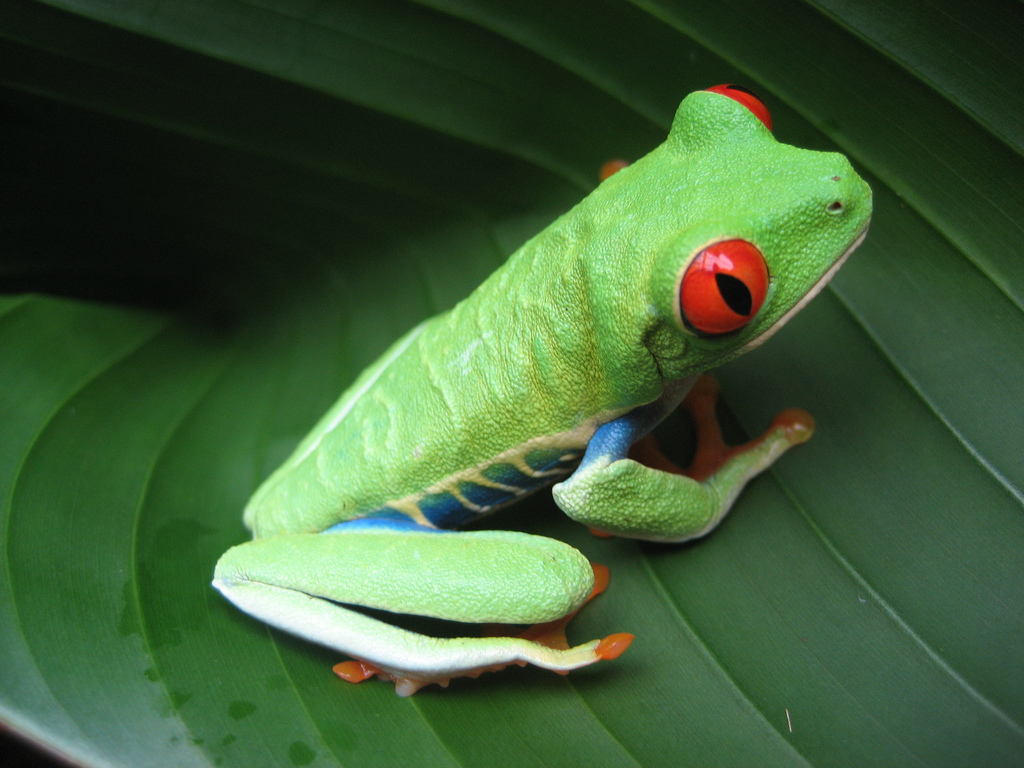
\includegraphics[width=.8\linewidth]{frog.jpg}
\caption{Placeholder image of a frog with a long example caption to show justification setting.}
\label{fig:frog}
\end{figure}

\subsection*{Digital Figures}
\label{sec:figures}

Only TIFF, EPS, and high-resolution PDF for Mac or PC are allowed for figures that will appear in the main text, and images must be final size. Authors may submit U3D or PRC files for 3D images; these must be accompanied by 2D representations in TIFF, EPS, or high-resolution PDF format.  Color images must be in RGB (red, green, blue) mode. Include the font files for any text. 

Figures and Tables should be labelled and referenced in the standard way using the \verb|\label{}| and \verb|\ref{}| commands.

Figure \ref{fig:frog} shows an example of how to insert a column-wide figure. To insert a figure wider than one column, please use the \verb|\begin{figure*}...\end{figure*}| environment. Figures wider than one column should be sized to 11.4 cm or 17.8 cm wide.

\subsection*{Single column equations}

Authors may use 1- or 2-column equations in their article, according to their preference.

To allow an equation to span both columns, options are to use the \verb|\begin{figure*}...\end{figure*}| environment mentioned above for figures, or to use the \verb|\begin{widetext}...\end{widetext}| environment as shown in equation \ref{eqn:example} below.

Please note that this option may run into problems with floats and footnotes, as mentioned in the \href{http://texdoc.net/pkg/cuted}{cuted package documentation}. In the case of problems with footnotes, it may be possible to correct the situation using commands \verb|\footnotemark| and \verb|\footnotetext|.

%% Do not use widetext if paper is in single column.
\begin{widetext}
\begin{align*}
(x+y)^3&=(x+y)(x+y)^2\\
       &=(x+y)(x^2+2xy+y^2) \numberthis \label{eqn:example} \\
       &=x^3+3x^2y+3xy^3+x^3. 
\end{align*}
\end{widetext}

\begin{table}%[tbhp]
\centering
\caption{Comparison of the fitted potential energy surfaces and ab initio benchmark electronic energy calculations}
\begin{tabular}{lrrr}
Species & CBS & CV & G3 \\
\midrule
1. Acetaldehyde & 0.0 & 0.0 & 0.0 \\
2. Vinyl alcohol & 9.1 & 9.6 & 13.5 \\
3. Hydroxyethylidene & 50.8 & 51.2 & 54.0\\
\bottomrule
\end{tabular}

\addtabletext{nomenclature for the TSs refers to the numbered species in the table.}
\end{table}

\subsection*{Supporting Information (SI)}

The main text of the paper must stand on its own without the SI. Refer to SI in the manuscript at an appropriate point in the text. Number supporting figures and tables starting with S1, S2, etc. Authors are limited to no more than 10 SI files, not including movie files. Authors who place detailed materials and methods in SI must provide sufficient detail in the main text methods to enable a reader to follow the logic of the procedures and results and also must reference the online methods. If a paper is fundamentally a study of a new method or technique, then the methods must be described completely in the main text. Because PNAS edits SI and composes it into a single PDF, authors must provide the following file formats only.

\subsubsection*{SI Text}

Supply Word, RTF, or LaTeX files (LaTeX files must be accompanied by a PDF with the same file name for visual reference).

\subsubsection*{SI Figures}

Provide a brief legend for each supporting figure after the supporting text. Provide figure images in TIFF, EPS, high-resolution PDF, JPEG, or GIF format; figures may not be embedded in manuscript text. When saving TIFF files, use only LZW compression; do not use JPEG compression. Do not save figure numbers, legends, or author names as part of the image. Composite figures must be pre-assembled.

\subsubsection*{3D Figures}

Supply a composable U3D or PRC file so that it may be edited and composed. Authors may submit a PDF file but please note it will be published in raw format and will not be edited or composed.

\subsubsection*{SI Tables}

Supply Word, RTF, or LaTeX files (LaTeX files must be accompanied by a PDF with the same file name for visual reference); include only one table per file. Do not use tabs or spaces to separate columns in Word tables.

\subsubsection*{SI Datasets} 

Supply Excel (.xls), RTF, or PDF files. This file type will be published in raw format and will not be edited or composed. 

\subsubsection*{SI Movies}

Supply Audio Video Interleave (avi), Quicktime (mov), Windows Media (wmv), animated GIF (gif), or MPEG files and submit a brief legend for each movie in a Word or RTF file. All movies should be submitted at the desired reproduction size and length. Movies should be no more than 10 MB in size. 

\subsubsection*{Still images}

Authors must provide a still image from each video file. Supply TIFF, EPS, high-resolution PDF, JPEG, or GIF files. 

\subsubsection*{Appendices}

PNAS prefers that authors submit individual source files to ensure readability. If this is not possible, supply a single PDF file that contains all of the SI associated with the paper. This file type will be published in raw format and will not be edited or composed.

\matmethods{Please describe your materials and methods here. This can be more than one paragraph, and may contain subsections and equations as required. Authors should include a statement in the methods section describing how readers will be able to access the data in the paper. 

\subsection*{Subsection for Method}
Example text for subsection.
}

\showmatmethods % Display the Materials and Methods section

\acknow{Please include your acknowledgments here, set in a single paragraph. Please do not include any acknowledgments in the Supporting Information, or anywhere else in the manuscript.}

\showacknow % Display the acknowledgments section

% \pnasbreak splits and balances the columns before the references.
% If you see unexpected formatting errors, try commenting out this line
% as it can run into problems with floats and footnotes on the final page.
\pnasbreak

% Bibliography
\bibliography{pnas-sample}

\end{document}